%%%%%%%%%%%%%%%%%%%%%%%%%%%%%%%%%%%%%%%%%%%%%%%%%%%%%%%%%%%%%%%%%%%%
%%%%%%%%%%%%%%%%%%%%%%%%%% PREMIÈRE PARTIE %%%%%%%%%%%%%%%%%%%%%%%%%
%%%%%%%%%%%%%%%%%%%%%%%%%%%%%%%%%%%%%%%%%%%%%%%%%%%%%%%%%%%%%%%%%%%%

\part{Du document numérisé au \xmltei: nature du corpus, structure des documents et méthode de production des données}
\chapter{Le marché des manuscrits autographes au prisme des catalogues de vente}
\chaptermark{Le marché des manuscrits autographes}
Ce chapitre présente l'objet d'étude du projet \mss{} : étudier le marché des manuscrits autographes du \scl{XIX}. parisien à partir de ses catalogues de vente et étudier la construction du canon littéraire au prisme du marché du manuscrit.

\section{Pourquoi étudier le marché des manuscrits autographes?}
Cette section porte sur l'intérêt scientifique des objets d'étude du projet (marché des manuscrits et étude de la construction du canon).


\section{La structure du corpus : périodisation, producteurs des documents et classification}
Ici est faite une présentation des documents traités dans le cadre du projet MSS. La présentation est à deux niveaux: au niveau du corpus et des catalogues. Ce chapitre s'appuie sur les mémoires effectués par d'ancien.ne.s stagiaires de \ktb{}, qui ont déjà beaucoup analysé la nature et les enjeux du corpus\footcite{rondeau_du_noyer_encoder_2019, corbieres_du_2020, janes_du_2021}.

\subsection{Le corpus de catalogues de vente de manuscrits}
Ici est présenté le corpus: nature, quantité de documents (et d'entrées individuelles), dates, différentes classifications qui peuvent être faites (revues, catalogues de ventes aux enchères ou à prix fixes...).

\subsection{Structure des catalogues}
% Ici sera présentée la structure des catalogues; la structure de chaque page ne sera détaillée qu'à la partie suivante.
=> zoupiloup on fait passer ça à la partie suivante

\chapter{Production des données: de l'OCR à la \tei{}}
\chaptermark{Production des données}
% Cette partie s'attache autant à présenter le processus d'\gls{océrisation} (qui est déjà bien établi et ne constitue pas le cœur de mon stage) que la structure des documents. Alors que le chapitre précédent s'intéresse aux catalogues dans leur ensemble, ici, on étudie le corpus au niveau de la page et de l'entrée individuelle. En effet, l'\gls{océrisation} repose sur la segmentation, et donc sur l'établissement d'une structure \enquote{abstraite} d'une page (c'est-à-dire, d'un découpage de la page en zones).
À la base de l'étude des catalogues de vente de manuscrits se trouve la production de données: les imprimés en tant que tels peuvent être analysés par une personne humaine, mais ne sont pas manipulables par une machine. Il est donc nécessaire d'extraire le texte des catalogues. Ce texte extrait, afin d'être manipulable par une machine, doit être ensuite conservé dans un format structuré et hiérarchisé, qui permette d'accéder facilement aux différentes entrées de catalogue, et aux différentes parties de ces entrées. Avant de pouvoir manipuler et analyser le texte, il est donc nécessaire de l'extraire, de le modéliser et de l'encoder en un format qui permette la mise au point de méthodes computationnelles. Cet encodage est le fruit d'une sélection et d'une interprétation des catalogues: certaines caractéristiques de ceux-ci sont privilégiées et d'autres sont abandonnées afin de parvenir à une édition numérique qui soit manipulable par une machine.

\section{Extraire le texte des imprimés: la transcription des catalogues}
Après avoir présenté le processus d'encodage en général, cette section décrit la structure des catalogues au niveau du document complet, de la page et de l'entrée ainsi que la manière dont les pages de catalogues sont segmentées en utilisant \textit{SegmOnto}. Cet intérêt pour la structure des catalogues est essentiel, puisque c'est cette structure qui permet de les modéliser, et donc de préparer leur édition en \xmltei{}.

\subsection{Une chaîne de traitement pour la transcription du texte}
L'extraction du texte des catalogues repose fortement sur \textit{eScriptorium}, une application en ligne de transcription\footcite{stokes_escriptorium_2021}. Elle permet la transcription manuelle ou automatisée de documents et est particulièrement utilisée pour entraîner des modèles de \gls{ocr}. En effet, l'entraînement d'un tel modèle se fait en produisant de la vérité de terrain, c'est-à-dire des documents transcrits à la main que le modèle pourra \enquote{apprendre} à reconnaître. L'application offre une interface graphique (visible en annexes \ref{appendix:escriptorium}) à \textit{Kraken}, un moteur de reconnaissance optique de caractères qui supporte un très grand nombre d'alphabets (latin, grec, arabe...). Elle est développée depuis 2018 à l'EPHE comme remplacement à \textit{Transkribus}. Cette seconde plateforme de transcription a un fonctionnement analogue, mais fonctionne sur un modèle propriétaire. Non seulement le code source de l'application et de son moteur d'\gls{ocr} ne sont pas accessibles, mais les modèles entraînés par les utilisateur.ice.s de \textit{Transkribus} ne peuvent être accédés directement. Cela rend impossible l'utilisation d'un tel modèle en dehors de l'application. En utilisant \textit{eScriptorium}, au contraire, l'extraction du texte des catalogues a un double intérêt: tout d'abord, elle permet de produire des données à traiter; ensuite, elle permet de produire de la vérité de terrain pour entraîner et améliorer les modèles d'\gls{ocr}.

L'extraction du texte est faite de façon semi-automatisée: une étape automatique est suivie d'une correction manuelle. Dans un premier temps, le texte est extrait automatiquement des catalogues grâce à un modèle d'\gls{ocr} pour les imprimés de l'époque contemporaine. Celui-ci est développé depuis des années, notamment à partir des catalogues de vente de manuscrits du projet \ktb{}\footcite[p. 34-35]{janes_du_2021}. Une fois ce texte extrait, une phase de correction manuelle des données est nécessaire: puisque les entrées de catalogue sont retraitées et diffusées sur un site internet, elles ne doivent pas contenir d'erreurs. Dans un premier temps, les différentes zones de texte doivent être définies. Cette segmentation de la page en différentes parties est également entreprise par \textit{eScriptorium}. Cependant, cette segmentation unifie les zones de texte dans des polygones, sans distinguer les différences ou hiérarchies qui peuvent exister dans une zone de texte, comme cela apparaît dans l'exemple \ref{fig:seg}. La segmentation de la page est donc refaite manuellement, en utilisant le vocabulaire \textit{SegmOnto}, comme cela est décrit plus bas. Il faut ensuite corriger les données elles-mêmes, c'est-à-dire reprendre manuellement la transcription afin de s'assurer qu'elle corresponde au texte. Une fois que les catalogues ont été transcrits, cette transcription est exportée en \alto{}. Ce format \xml{} reproduit la structure physique d'un document en associant à chaque ligne de texte sa position sur la page en pixels. Ce format est ensuite transformé pour produire des fichiers \xmltei{}, un format qui permet l'encodage d'un catalogue entier. La \tei{} permet, comme cela est expliqué plus tard, un encodage sémantique d'un document entier, et non la relation entre le texte et le document dont il est transcrit. Dans le projet \mssktb{}, la conversion de l'\alto{} en \tei{} était originellement faite grâce à \textit{GROBID-Dictionnaries}, un outil produisant des fichiers \tei{} sur mesure pour des catalogues\footcite{khemakhem_automatically_2018}. Cet outil, basé sur l'intelligence machine, n'est plus en usage par le projet; il est en train d'être remplacé par des méthodes plus simples, basées sur la détection de motifs dans le texte.

\begin{figure}[h]
	\centering
	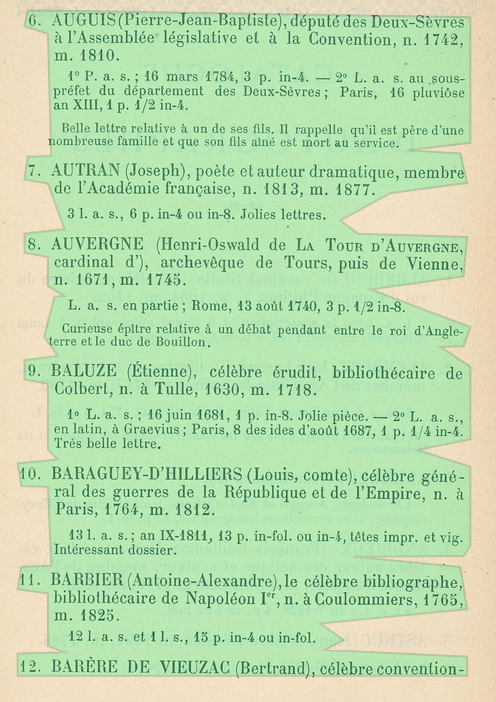
\includegraphics[width=0.4\textwidth]{img/cat_000445_p2}
	\caption{Exemple de segmentation automatique par \textit{eScriptorium}}
	\label{fig:seg}
\end{figure}


\subsection{Comprendre la structure du document pour préparer l'édition numérique}
L'encodage numérique d'un document se doit, autant que possible, d'être représentatif du document originel ou de certains aspects de celui-ci qui sont considérés comme importants en fonction des objectifs scientifiques du projet. La première étape de l'encodage est donc de comprendre la structure de ce qui sera encodé. Comme celrick rossa a été dit, plusieurs typologies de documents existent; dans le cadre de mon stage, la production de données s'est concentrée sur les catalogues de ventes aux enchères organisées par Étienne Charavay. C'est donc à partir de la structure de ceux-ci que s'appuie la présentation qui suit.

\subsubsection{La structure des catalogues}
L'encodage numérique repose sur des choix scientifiques: il n'est pas possible d'encoder toutes les caractéristiques possibles d'un document. Il est donc nécessaire de faire des choix qui privilégient les enjeux scientifiques du projet; ces choix se reflètent dans ce qui est conservé et ce qui ne l'est pas au sein  des documents. Le projet \mssktb{} choisit une orientation particulière, qui se concentre sur les manuscrits en vente dans les catalogues\footcite[p. 27]{rondeau_du_noyer_encoder_2019}. Cela implique donc que certaines pages de catalogues ne sont pas retranscrites ni encodées. Dans les revues-catalogues à prix marqués, par exemple, les pages contenant des articles et des réclames ne sont pas retranscrites. D'abord, leur retranscription ne servirait pas les objectifs du projet. Mais de plus, ces pages, qui contiennent des images, sont trop homogènes pour le processus de reconnaissance optique de caractères. En effet, un tel processus repose sur l'entraînement d'un logiciel qui \enquote{apprend} à reconnaître des caractères dans un texte numérisé. Ce logiciel ne pouvant par défaut pas faire la distinction entre le texte et les parties graphiques des catalogues, il cherche à interpréter les illustrations comme du texte. Il est donc important de faire la différence entre la structure du document réel, tel qu'il est conservé par une bibliothèque, et la structure retenue pour ce projet, qui ne contient que les pages de catalogue considérées comme étant utiles. La page de titre d'un catalogue est retenue pour deux raisons: elle permet d'identifier celui-ci et offre des données bruitées (puisque cette page contient des motifs graphiques), qui sont utiles pour entraîner le logiciel de reconnaissance de caractères. Les catalogues de vente aux enchères contiennent également une ou deux pages introductives (qui présentent la vente et d'autres ouvrages publiés par l'éditeur). Celles-ci sont transcrites, là encore pour produire des données bruitées. Les pages de conclusion (qui contiennent notamment une liste de publications de l'éditeur) ne sont pas retranscrites. Le corps d'un catalogue est fait de pages listant les manuscrits en vente. Ces pages sont la source des données utilisées par \mssktb{}, et sont donc décrites ci-dessous.

Comme cela apparaît dans la figure \ref{fig:catpage}, la structure des pages de catalogues présente une grande régularité. La page de gauche présentée ici fait partie des quelques pages \enquote{spéciales} qui sont contenues dans les catalogues, puisque c'est la première page listant les items en vente. Elle débute donc par un bandeau décoratif et un titre dans une police plus grande que le reste de la page. Les autres pages listant des pièces en vente ont une structure plus homogène, puisqu'elles ne contiennent ni d'éléments graphiques ni de différence dans les fontes utilisées. La structure de la majorité des pages de catalogues ressemble donc à la page de droite dans la figure \ref{fig:catpage}. Les entrées se succèdent les unes après les autres; chaque entrée de catalogue étant numérotée, le début d'une nouvelle entrée est facilement identifiable grâce à son identifiant numéraire.

\begin{figure}[h]
	\centering
	\begin{subfigure}{0.45\textwidth}
		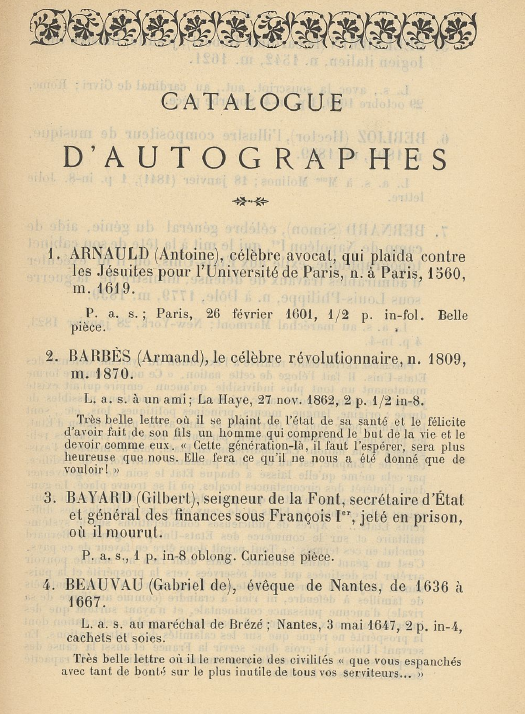
\includegraphics[width=\textwidth]{img/CAT_000441_0.png}
	\end{subfigure}
	\begin{subfigure}{0.45\textwidth}
		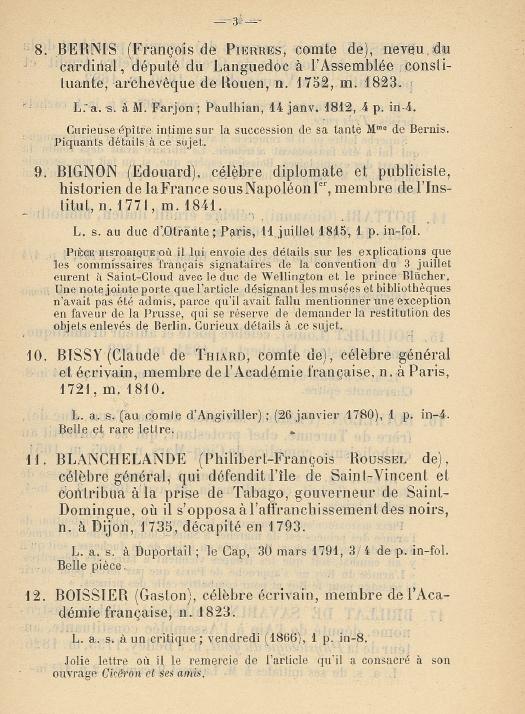
\includegraphics[width=\textwidth]{img/CAT_000441_1.png}
	\end{subfigure}
	\caption{Deux pages de catalogues de ventes aux enchères (\textit{Catalogue d'une précieuse collection de lettre autographes}, vente Étienne Charavay, 20 mai 1890)}
	\label{fig:catpage}
\end{figure}

\subsubsection{Appréhender la structure de la page à l'aide de SegmOnto}
% La structure des catalogues est présentée au niveau de la page. L'ontologie SegmOnto\footcite{christensen_segmonto_2022} est utilisée, autant pour appréhender la structure de la page que pour exprimer cette structure de façon standardisée.
La segmentation de la page en zones est une tâche centrale dans la transcription de documents. Elle est définie par Antonacopoulos et al. (2011, cité.e.s par Thibault Clérice\footcite[p. 4]{clerice_you_2022}) comme l'identification de zones de textes sur une page (la segmentation en tant que telle) et la classification de ces zones en fonction de leur contenus. La segmentation a tout d'abord une utilité \enquote{intellectuelle}: elle permet de mieux comprendre comment les contenus d'un document s'organisent sur une page. L'analyse de la disposition des informations sur une page est en fait la manière dont un.e lecteur.ice aborde un document\footcite{christensen_segmonto_2022}. Ce processus a également un rôle essentiel pour l'automatisation de la transcription automatique: la détection des zones de texte est une étape préalable à la reconnaissance des caractères. De plus, expliciter la distinction entre les différentes parties de la page permet, ultérieurement, de filtrer les différentes parties du texte pour ne conserver que celles qui sont pertinentes. Cela est particulièrement utile dans le domaine de la \gls{ocr}. Si un document contient dans sa partie centrale de l'imprimé et dans ses marges du texte manuscrit et que les deux parties sont transcrites, l'entraînement d'un modèle sur ce document aura des résultats pour le moins problématiques. Le modèle apprendra en effet à identifier deux formes d'écritures très différentes comme étant la même. C'est ici que le zonage du texte est pertinent: il permet, par exemple, de ne conserver que le texte principal, et donc de diminuer le bruit présent dans les données.

La segmentation des zones faite automatiquement par \textit{Kraken} est reconnue comme étant une faiblesse de ce moteur d'\gls{ocr}\footcite[p. 1]{clerice_you_2022}. Celle-ci se base sur la construction d'un ou de plusieurs polygones pour englober le texte d'une page (\ref{fig:seg}). Les différentes zones ne sont pas perçues comme ayant une fonction différente dans le texte, et Kraken a tendance à agglomérer dans un seul polygone des zones de texte qui devraient être considérées de façon distinctes. C'est le cas dans l'exemple \ref{fig:seg}, où tout le corps de la page est intégré dans une seule zone de texte. La segmentation faite par Kraken ne correspond donc pas avec les besoins de la production de vérité de terrain. Aussi doit-elle être remplacée. Des méthodes alternatives ont été développées permettant une segmentation plus qualitative de documents, comme \textit{YALTAi}\footcite{clerice_you_2022}, qui s'appuie sur des méthodes de reconnaissance des formes. Cet outil n'était pas encore fonctionnel lors de la phase de transcription de documents de mon stage; aussi la segmentation des catalogues a-t-elle été faite manuellement.

Segmenter un texte manuellement n'est pas difficile; la classification des zones, cependant, ne peut être faite en utilisant un vocabulaire \enquote{fait maison}: une vérité de terrain n'est réutilisable par d'autres que si le texte retranscrit est segmenté de façon compréhensible. Dans un souci d'interopérabilité, la définition de zones dans la page a donc été fait à l'aide de \textit{SegmOnto}, une ontologie pour la segmentation de documents\footcite{christensen_segmonto_2022, gabay_segmonto_2021}. Utiliser un vocabulaire commun à plusieurs projets est un moyen de rendre les données produites plus facilement compréhensibles par d'autres et de faciliter leur réutilisation par d'autres projets de recherche. \textit{SegmOnto} définit un vocabulaire permettant une segmentation sémantique des document, c'est-à-dire un découpage qui explicite le rôle des différentes parties de la page. Le projet a développé une approche matérielle des documents\footcite{gabay_segmonto_2021} qui cherche à définir un vocabulaire commun et simple pour segmenter la plus grande quantité de manuscrits possibles. Ce vocabulaire est conçu de façon modulaire: chaque zone doit appartenir à un \enquote{type}, c'est-à-dire à un terme issu d'un vocabulaire contrôlé; l'un de ces termes est \enquote{CustomZone}, qui permet de définir des zones n'appartenant pas à \textit{SegmOnto}. Ces différents types peuvent de plus être précisés grâce à des sous-types (qui sont librement définis par un projet); enfin, les zones peuvent être hiérarchisées entre elles. Une zone conforme à \textit{SegmOnto} doit donc correspondre à l'expression suivante: \texttt{type(:sous-type)?(\#\textbackslash{}d)?} (soit un type suivi d'un sous-type optionnel et d'une hiérarchisation optionnelle).

\textit{SegmOnto} définit un vocabulaire simple à la finalité pratique: pouvoir filtrer les différentes parties d'une page pour entraîner des modèles d'\gls{ocr} sur des données propres. Par conséquent, l'utilisation de \textit{SegmOnto} pour structurer des catalogues de vente de manuscrits est elle aussi simple. Les éléments utilisés sont les suivants:

\begin{itemize}
	\item \texttt{MainZone}: cet zone correspond à la partie principale d'une page.
	\item \texttt{TitlePageZone}: cette zone identifie la partie principale de la page de titre. Elle est utilisée sur la page de titre à la place de \texttt{MainZone} car la page de titre contient de nombreux éléments graphiques, alors que la partie principale des autres pages n'en contient pas.
	\item \texttt{GraphicZone}: cette zone permet de contenir des éléments graphiques qui doivent être distingués du corps du texte.
	\item \texttt{RunningTitltZone} est une zone permettant d'indiquer la présence d'un titre courant.
	\item \texttt{MarginTextZone}: l'usage de cette zone permet de contenir des signatures et autres notes manuscrites en marge du texte.
	\item \texttt{CustomZone:Entry} est une zone propre au projet \mssktb{} qui permet de désigner une entrée de catalogue.
	\item \texttt{CustomZone:EntryEnd} est utilisée lorsqu'une entrée de catalogue se poursuit sur plus d'une page: elle sert à indiquer qu'une entrée a été débutée à la fin de la page précédente.
\end{itemize}

À l'aide de ces sept éléments (dont deux qui n'ont pas été définis par \textit{SegmOnto}), il est possible d'annoter l'intégralité des catalogues. Comme cela apparaît dans les exemples \ref{fig:catzones}, les éléments utilisés diffèrent beaucoup en fonction de la page qui est segmentée. Les pages contenant des items en vente (\ref{fig:catp1}, \ref{fig:catp2}) sont majoritairement composées d'une \texttt{MainZone} contenant des \texttt{CustomZone:Entry} et \texttt{CustomZone:EntryEnd}. La première de ces deux pages est également la première page du catalogue, et elle contient donc également un \texttt{RunningTitleZone}, ainsi qu'un \texttt{GraphicZone}. La segmentation de la page de titre (\ref{fig:cattitle}) diffère beaucoup des autres pages du catalogue. La page de titre contient beaucoup d'éléments graphiques; pour la distinguer des autres pages, elle est donc contenue dans un \texttt{TitlePageZone}. Elle peut également être complétée de signatures, ou de notes manuscrits; ici, une signature est contenue dans un \texttt{MarginTextZone}.

\begin{sidewaysfigure}[p]
	\begin{subfigure}{0.33\textwidth}
		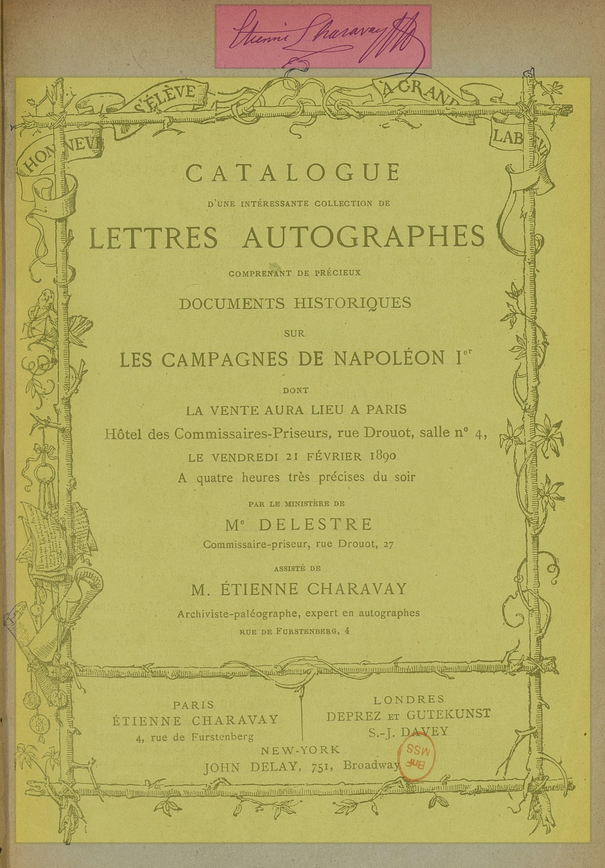
\includegraphics[width=\textwidth]{img/cat_000434_couv_zones.png}
		\caption{La page de titre}
		\label{fig:cattitle}
	\end{subfigure}
	\begin{subfigure}{0.33\textwidth}
		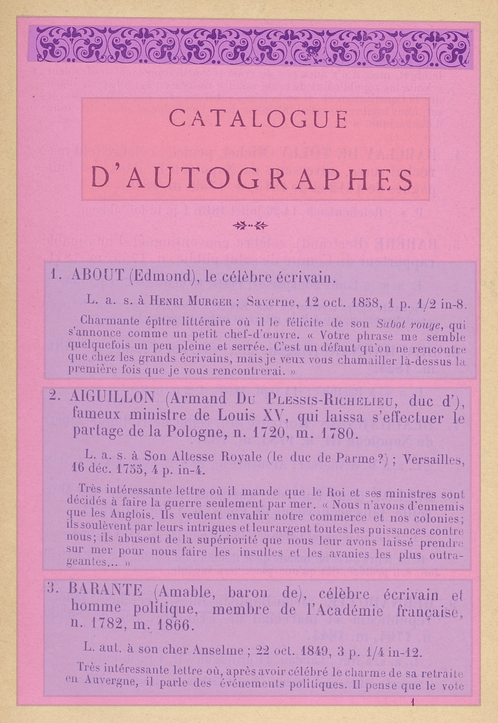
\includegraphics[width=\textwidth]{img/cat_000434_p1_zones.png}
		\caption{La première page du catalogue}
		\label{fig:catp1}
	\end{subfigure}
	\begin{subfigure}{0.33\textwidth}
		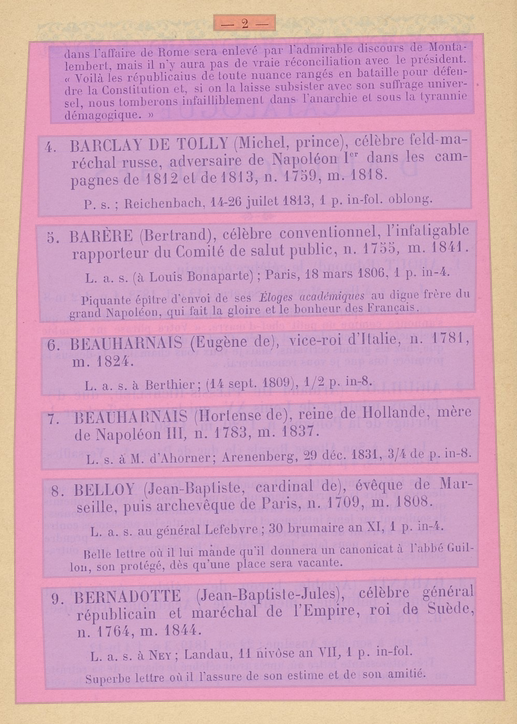
\includegraphics[width=\textwidth]{img/cat_000434_p2_zones.png}
		\caption{La seconde page du catalogue}
		\label{fig:catp2}
	\end{subfigure}
	\caption{La segmentation de trois pages de catalogues de ventes aux enchères (\textit{Catalogue d'une précieuse collection de lettre autographes}, vente Étienne Charavay, 21 février 1890)}
	\label{fig:catzones}
\end{sidewaysfigure}

Si cette segmentation n'est pas réutilisée dans une fois que les fichiers \alto{} ont été convertis en \tei{}, cette étape est néamoins importante. D'abord, elle garantit que la recherche produite par \mssktb{} soit réutilisable par d'autres projets, puisque l'utilisation de \textit{SegmOnto} permet que la vérité de terrain produite soit réutilisable. Ensuite, le découpage des pages de catalogues en zones met également en avant une unité intellectuelle pour les catalogues: celle des items vendus. Mettre en avant l'item comme élément structurant marque un éloignement des catalogues papiers, où la page c'est la page qui joue un rôle d'importance. Au contraire, les catalogues encodés ne gardent pas mention des pages, mais prennent pour élément central les entrées individuelles.


\subsubsection{Description des entrées de catalogue: préparer l'édition \tei{}}
% Ici, la structure des catalogues est présentée au niveau de l'entrée, c'est à dire du lot mis en vente. C'est à autour de la structure des entrées qu'est construite l'édition \xmltei{}. On s'intéresse à la structure des entrées individuelles à deux niveaux:
% \begin{itemize}
%	\item Au niveau intellectuel: quelles sont les différentes parties d'une entrée (titre, description du manuscrit, prix...).
%	\item Au niveau  \enquote{textuel}: quels sont les séparateurs, c'est à dire les éléments dans le texte qui permettent de séparer les pages de catalogue en entrées et les entrées en sous-éléments) correspondant à la structure intellectuelle décrite ci-dessus.
%\ end{itemize}

Au niveau de l'entrée, les catalogues de vente présentent la même régularité: chaque item en vente est décrit de façon analogue à ce qui est visible en \ref{fig:catitem}. Après le numéro de l'item se trouve le nom de l'auteur.ice du manuscrit ainsi qu'une description succincte de cette personne. Il arrive que, à la place du nom de l'auteur soit utilisé une titre comme \enquote{Documents divers} ou la mention d'un évènement historique (\enquote{Révolution française}). Lorsque c'est avec le nom d'une personne que débute une entrée de catalogue, celui-ci est souvent composé d'un nom de famille complet ainsi que d'un prénom, abrégé ou non. Celui-ci est souvent entre parenthèses et aprestès le nom de famille. La description mentionne quelques faits biographiques. Dans la grande majorité des cas, ceux-ci se concentrent sur l'occupation de la personne, sa date de naissance et de décès; parfois, la façon dont une personne est morte peut également être décrite. Ensuite se trouve une description de l'item en vente lui-même (\enquote{L. a. s. au citoyen Victor Delaunay...}). Cette description, pour des raisons d'économie d'espace, s'appuie sur un vocabulaire et une structure très codifiée, avec de nombreuses abréviations. D'abord est indiqué le type de lettre (\enquote{L. a. s.}, pour \enquote{Lettre autographe signée}). Dans le cas d'une lettre est également indiqué le ou la destinataire ainsi que le lieu et la date où celle-ci a été écrite. Après cette description très succincte et normée se trouve parfois un paragraphe additionnel donnant des détails sur les lettres, comme c'est le cas dans cet exemple. C'est en général dans ce paragraphe qu'est indiqué le sujet du manuscrit, ainsi que, parfois, un extrait de celui-ci. Lorsqu'un manuscrit est vendu à prix fixe, alors ce prix est également indiqué à la fin de l'entrée.

\begin{figure}[h]
	\centering
	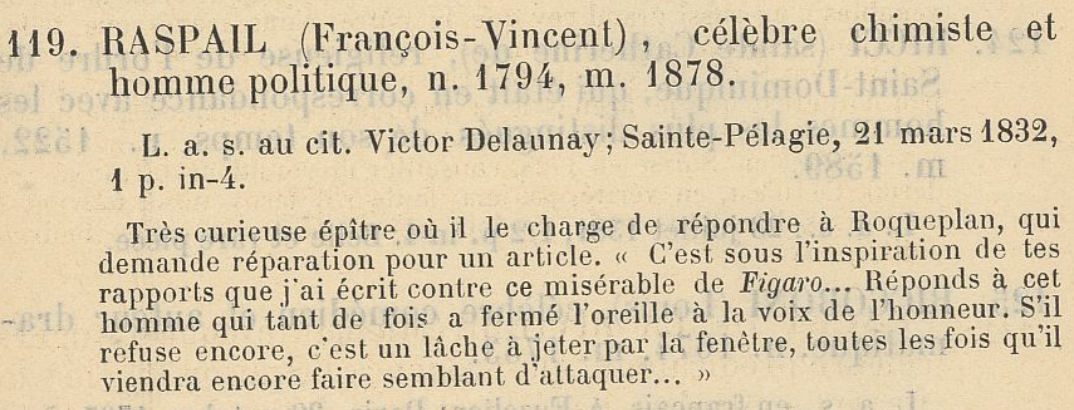
\includegraphics[width=\textwidth]{img/CAT_000441_e119}
	\caption{Une entrée de catalogue (\textit{Catalogue d'une précieuse collection de lettre autographes}, vente Étienne Charavay, 20 mai 1890)}
	\label{fig:catitem}
\end{figure}

Il apparaît donc que les catalogues de vente de manuscrits ont toujours une structure très rigide, aussi bien au niveau de l'ensemble du catalogue, que de la page et même de l'entrée. Des sauts de ligne marquent la différence entre les entrées et, dans les catalogues de ventes d'Étienne Charavay, des sauts de ligne distinguent également les différentes parties d'une entrée. D'autres caractères typographiques permettent d'établir des séparations supplémentaires entre les différentes informations présentes. Par exemple, le prénom est distinct du nom de famille à l'aide de parenthèses; une virgule distingue la description de l'auteur.ice de son nom. Enfin, à l'exception du paragraphe contenant des détails additionnels et du prix, tous les catalogues contiennent les mêmes informations. Il est donc possible de définir un modèle abstrait qui soit à même de représenter tous les catalogues (\ref{fig:catmodel}). Ce modèle peut servir de base pour structurer les données extraites des catalogues afin qu'elles soient manipulables; cependant, il reste un long processus pour arriver à ces données structurées.

\begin{figure}[h]
	\centering
	\tikz[scale=0.85,transform shape]{
		\node[base] (cat) at (0,0)%
		{Catalogue};
		\node[base] (intro) at (-5,-2)%
		{Titre et pages introductives};
		\node[base] (main) at (0,-2)%
		{Entrées de catalogues};
		\node[base] (conclu) at (5,-2)
		{Pages de fin};
		\node[base] (tname) at (-7.5,-4)%
		{Nom de l'auteur.ice};
		\node[base] (ttrait) at (-2.5,-4)%
		{Description de l'auteur.ice};
		\node[base] (tdesc) at (2.5,-4)%
		{Description du manuscrit};
		\node[base] (tnote) at (7.5,-4)%
		{Détails additionnels};
		\draw[arrow] (cat) -- (intro);
		\draw[arrow] (cat) -- (main);
		\draw[arrow] (cat) -- (conclu);
		\draw[arrow] (main) -- (tname);
		\draw[arrow] (main) -- (ttrait);
		\draw[arrow] (main) -- (tdesc);
		\draw[arrow] (main) -- (tnote);
	}
	\caption{Modèle d'un catalogue de vente de manuscrits}
	\label{fig:catmodel}
\end{figure}


\section{L'encodage des manuscrits en \xmltei{}}
\subsection{Encoder les catalogues en \tei{}}
Ici est présentée la représentation \xmltei{} des catalogues de vente.

\subsection{L'encodage en \tei{}: un processus sélectif qui réduit les significations du texte}
Après une étape d'\gls{océrisation} via \escr{}, le texte extrait des PDF peut être exporté soit en texte brut, soit en \xml{} \texttt{Page} ou \alto{}. Ces formats s'attachent à garder une relation entre le \xml{} et le document numérisé (les zones de texte sont indiquées, chaque ligne est dans une balise...). Cependant, l'unité intellectuelle centrale à la suite du projet, ce n'est pas la page numérisée, mais l'entrée de catalogue. Un format plus complexe que le \xml{} d'\escr{} est donc nécessaire. Assez logiquement, la suite du projet s'appuie sur une traduction des catalogues en \tei{}. On s'intéresse autant à la structure des documents \xml{} (quelles balises sont utilisées...) qu'à l'intérêt scientifique d'une édition numérique (balisage sémantique, possibilité de normaliser les informations grâce à des attributs).

L'édition numérique en \xmltei{} des catalogues implique une certaine perte d'informations: l'intégralité des significations contenues dans les catalogues imprimés ne peut être traduite en \tei{} (la police, ou la qualité du papier, peuvent être documentés mais ne peuvent pas être reproduites). Ce genre de perte d'information a lieu, à différents degrés, dans la plupart des éditions \tei{}: ce format n'est pas un substitut des documents originels. Dans le projet \mssktb{}, d'autres informations sont perdues: l'édition numérique n'est pas censée être une représentation exhaustive des catalogues. La \tei{} n'est pas utilisée comme un format de conservation, mais comme un format de traitement qui sera enrichi dans les différentes étapes. Afin de mesurer ce qui est conservé et ce qui est perdu du document originel, l'édition \tei{} sera analysée à la lumière de la \enquote{roue du texte} du philologue Patrick Sahle\footcite[p. 11]{sahle_digital_2016} qui modélise les significations plurielles d'un texte.

cf Smith+Blackwell (2012): texte (édition critique) peut être rpr sous la forme d'un graphe RDF de citations

parler aussi de l'OHCO (renear\_refining\_1996) et des critiques qui lui ont été faites dès les débuts de la TEI

John Frow + Susan Pearce ?